\documentclass[12pt]{article}
\usepackage{enumerate}
\usepackage{notes}

\begin{document}
\title{Oxford A1 - Differential Equations \footnotetext{\url{https://courses.maths.ox.ac.uk/node/5372}}}
\author{Dan Davison}
\maketitle

\section{Sheet 1}

\newpage
\subsection*{}
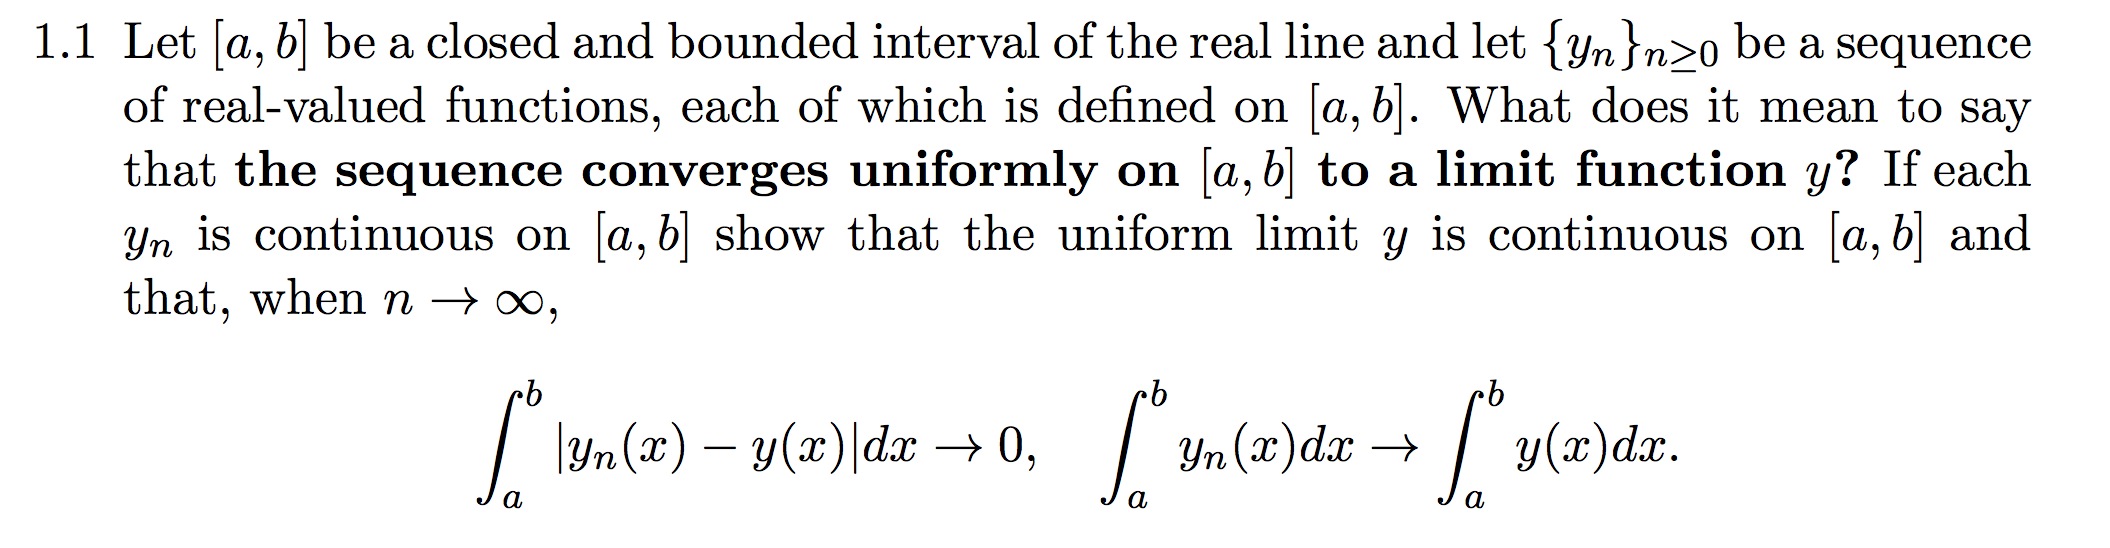
\includegraphics[width=450pt]{img/differential-equations-a1-1-1-a.png}\\
\begin{mdframed}
  \subsubsection*{(a) Definition of uniform convergence}
  The sequence of functions $\{y_n\}_{n\geq 0}$ \textbf{converges uniformly on
    $[a, b]$ to $y$} if and only if for every $\epsilon > 0$ there exists an
  $m \in \N$ such that for every $n > m$, $y_n$ differs from $y$ by no more
  than $\epsilon$ at every point in $[a,b]$.

  \subsubsection*{(b) Show that the limit function is continuous}

  The claim is that if each $y_n$ is continuous on $[a,b]$ then $y$ is
  continuous on $[a,b]$. We are told that
  \begin{enumerate}
  \item $\{y_n\}_{n \geq 0}$ converges uniformly to $y$, and
  \item each $y_n$ is continuous on $[a,b]$.
  \end{enumerate}

  % We need to show that for every $\epsilon > 0$, for every $x_0 \in [a, b]$,
  % there exists a $\delta > 0$ such that
  % $|x - x_0| < \delta \implies |y(x) - y(x_0)| < \epsilon$.

  Fix arbitrary $\epsilon > 0$ and $x_0 \in [a,b]$.

  Let $m \in \N$ be such that $|y_m(x_0) - y(x_0)| < \epsilon/3$. Such an $m$
  exists because the $\{y_n\}$ converge uniformly to $y$.

  Let $\delta$ be such that
  $|x - x_0| < \delta \implies |y_m(x) - y_m(x_0)| < \epsilon/3$. Such a
  $\delta$ exists because $y_m$ is continuous on $[a,b]$.

  Fix an arbitrary $x$ such that $|x - x_0| < \delta$.

  Now we have the following:
  \begin{enumerate}
  \item $|y(x_0) - y_m(x_0)| < \epsilon/3$ ~~~~ by convergence of the $\{y_n\}$
  \item $|y_m(x_0) - y_m(x)| < \epsilon/3$ ~~~ by continuity of $y_m$
  \item $|y_m(x) - y(x)| < \epsilon/3$    ~~~~~~ by convergence of the $\{y_n\}$
  \end{enumerate}
  Therefore $|y(x_0) - y(x)| < \epsilon$, proving continuity of $y$ on $[a,b]$. \qed

  \subsubsection*{(c) Show that the definite integrals converge}

\end{mdframed}

\newpage
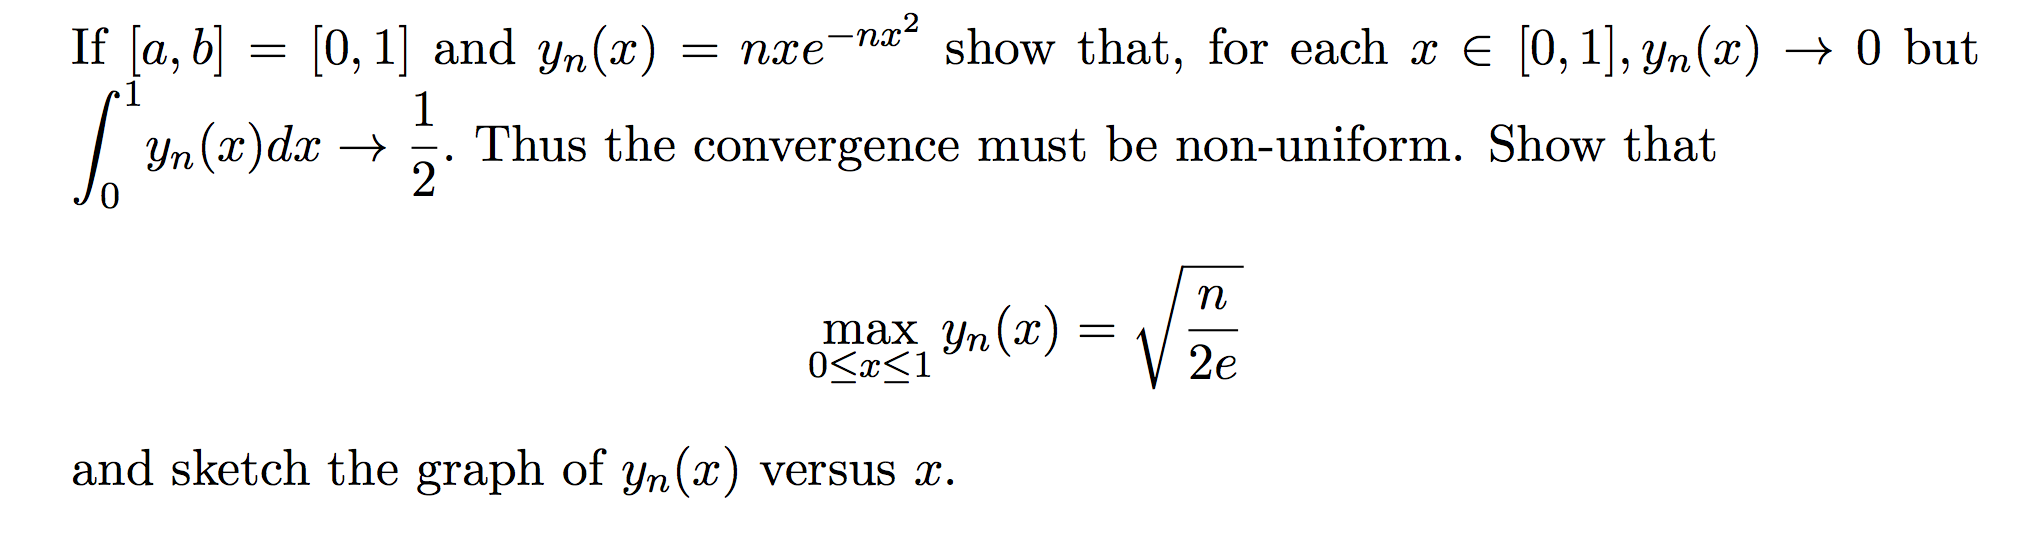
\includegraphics[width=450pt]{img/differential-equations-a1-1-1-b.png}\\
\begin{mdframed}
\end{mdframed}

\end{document}
